%%%%%%%%%%%%%%%%%%%%%%%%%%%%%%%%%%%%%%%%%%%%%%%%%%%%%%%%%%%%%
%% HEADER
%%%%%%%%%%%%%%%%%%%%%%%%%%%%%%%%%%%%%%%%%%%%%%%%%%%%%%%%%%%%%

\documentclass[a4paper, twocolumn, oneside, 10pt]{article}

\usepackage{fourier}
\usepackage[T1]{fontenc}

\usepackage{amssymb}
\usepackage{graphicx}
\usepackage{rotating}
\usepackage{pdflscape} 
\usepackage{abstract}
\usepackage[ table ]{ xcolor }
\usepackage[square, comma, sort&compress, longnamesfirst]{natbib} %
\usepackage{subfigure}
\usepackage{setspace}
%\singlespacing %% 1-spacing (default)s
%\onehalfspacing
\newcommand{\degree}{$^{\circ}$\ }
%%% END Article customizations

%%% The "real" document content comes below...

\title{The saccadic flow baseline: Accounting for task- and image-independent biases in fixation behaviour }

\author{Alasdair D. F. Clarke, Matthew J. Stainer, Ben Tatler \& Amelia R. Hunt}

\begin{document}

\twocolumn[
\maketitle
\begin{onecolabstract}
Much effort has been made to explain eye guidance during natural scene viewing. However, a substantial component of fixation placement appears to be a set of consistent biases in eye movement behaviour. We introduce the concept of saccadic flow, a generalisation of the central bias that described the image-independent conditional probability of making a saccade to $(x_{i+1},y_{i+1})$ given a fixation at $(x_i,y_i)$. We suggest that saccadic flow can be used as a useful prior when carrying out analysis into fixation locations, and can be used as a sub-module in models of eye movements during scene viewing. We demonstrate the utility of this idea by presenting bias-weighted gaze landscapes, and re-analyse some previous results to demonstrate how these ideas can be used. We also present a minor improvement to the central bias (based on using a multivariate truncated Gaussian), and investigate the leftwards and coarse-to-fine biases. 
\end{onecolabstract}
]

%%%%%%%%%%%%%%%%%%%%%%%%%%%%%%%%%%%%%%%%%%%%%%%%%%%%%%%%%%
\section{Introduction}
%%%%%%%%%%%%%%%%%%%%%%%%%%%%%%%%%%%%%%%%%%%%%%%%%%%%%%%%%%

The human fovea provides a small window of high acuity vision to the world, and as such the locations that we select to view through this window can tell us about how we seek the information necessary to complete the task we are currently undertaking. Fixation locations are selected based on a combination of low-level factors (such as visual salience \citep{itti-koch2000} or orientation information \citep{baddeley2006}) and high-level factors \citep{yarbus1967, buswell1935, land2001}. However, there are also strong observable biases in eye movements that are independent of the content of the scene or the task being performed  \citep{tatler2008, tatler2009, foulsham2010}, such as a strong tendency to fixate near to the centre of images \citep{tatler2007, canosa2003}. If we are to gain a complete understanding of the factors that govern how we sample information, we must build models of eye guidance on the framework of these underlying biases, using these as a baseline against which to compare effects of scene, task, and individual differences.

%%%%%%%%%%%%%%%%%%%%%%%%%%%%%%%%%%%%%%%%%%%%%%%%%%%%%%%%%%%%%
\subsection{Eye movement heuristics}
%%%%%%%%%%%%%%%%%%%%%%%%%%%%%%%%%%%%%%%%%%%%%%%%%%%%%%%%%%%%%

One of the most influential models of eye movements of the last decade is the optimal search model \citep{najemnik-geisler2008}, which posits that human saccadic behaviour during visual search is consistent with predictions made by an ideal observer. The number of fixations human observers needed to make to find the target was closely matched by the ideal observer model, in which successive fixations were selected based on reducing uncertainty about the target's location, taking into account search history and target visibility across the visual field. The efficiency of human search (at least, in search for a Gabor patch hidden in $1/f$-noise) suggests this as a plausible mechanism for selecting fixations during search.

While this modelling framework is attractive, there are several issues. The computations driving each fixation are complex, and depend on a fairly precise representation of one's own acuity over the visual field for a wide range of possible target/background combinations. One might therefore question the assumption that these computations are undertaken to determine the location of each of the 3-4 fixations made every second during visual search. More importantly,  \cite{morvan-maloney2012} demonstrated that human observers are not able to use information about visual sensitivity in the periphery to rationally plan even a a single saccade to the optimal location in a target discrimination task. In their experiment, the observer simply has to select a location from which to detect a target that can appear with equal probability in one of two possible locations. If the locations are relatively close together, a location in between the two possible locations will maximise the probability to detect a target appearing in either location. When the targets are too far apart to reliably detect the target from a point equidistant between them, the rational strategy is to look directly at one possible target location or the other. Inconsistent with optimal viewing strategies, however, the observers did not systematically modify their choice about where to fixate according to the distance between the possible target locations. This striking failure of optimality has recently been replicated in a larger sample and generalised to other decisions in addition to eye movements  \citep{clarke-hunt2015}. To reconcile their results with those of  \cite{najemnik-geisler2008},  \cite{morvan-maloney2012} suggest \textit{heuristics} guide saccade planning; that is, basic oculomotor biases such as a tendency to make saccades of particular amplitudes, and/or to particular regions of a display, or in particular sequences.  

This idea has recently been formalised and extended by \cite{clarke2015}, who demonstrate that a stochastic search model based on a memoryless random walk can find a target in noise in a similar number of fixations to human observers. The key component of this model was the use of the empirical distribution of saccades: for each saccade the model randomly samples a saccade from distributions estimating the likelihood a human observer made a saccade from $(x_{i+1},y_{i+1})$ to $(x_i,y_i)$. This stochastic model differs from the random baseline implemented by \cite{najemnik-geisler2008}, in which they randomly selected each fixation location from all possible points in the display, because it incorporates basic oculomotor heuristics that guide the eyes, without the need for complex computation of peripheral sensitivity or target location probability. In this paper, we re-implement and generalise this model, named \textit{saccadic flow}, and examine the extent to which it is useful as a prior for analysing eye movements made with more natural stimuli. This concept is illustrated in Figure \ref{fig:empiricalSaccadicFlow}. 
\begin{figure*}[htb]
\centering
\subfigure{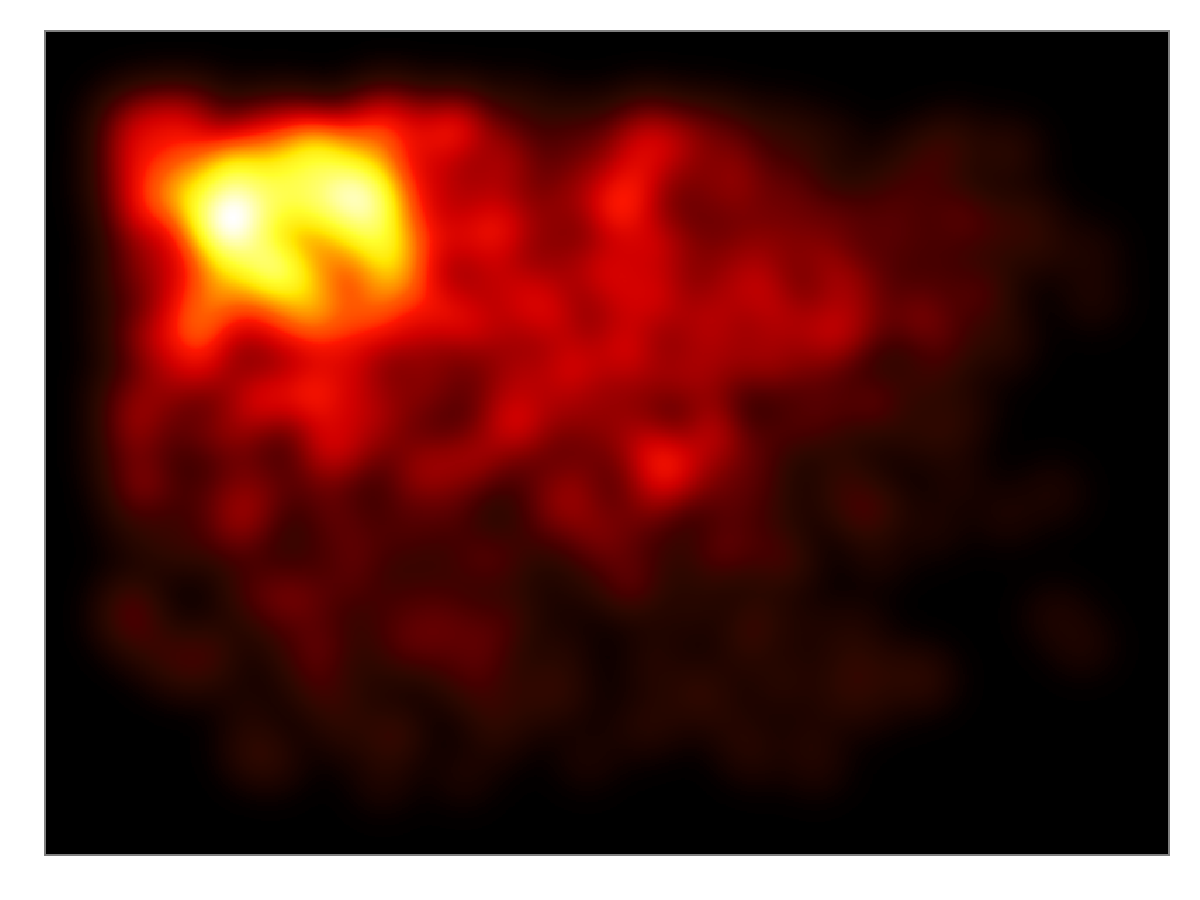
\includegraphics[width=4.2cm]{../scripts/heatmaps/SaccadicFlowMaps/Figures/BBias_11.pdf}}
\subfigure{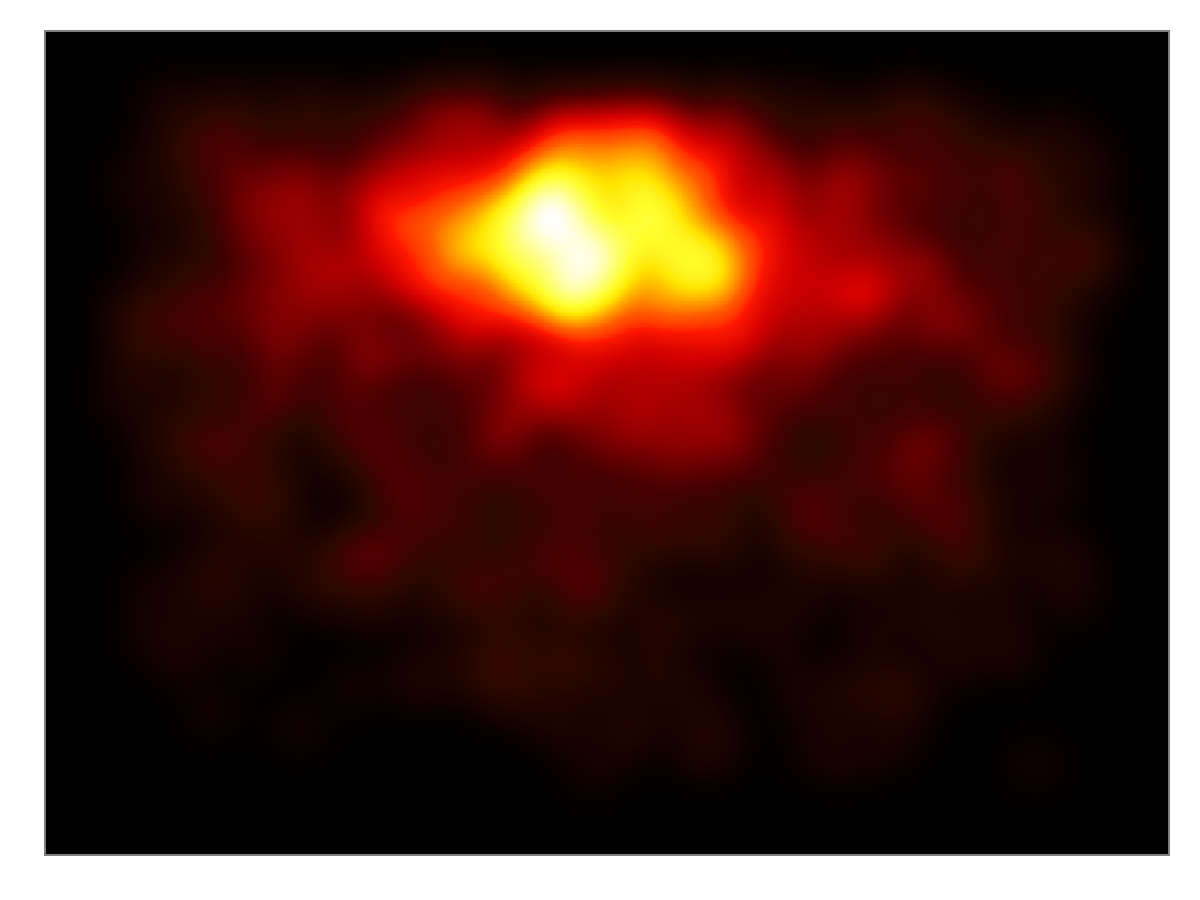
\includegraphics[width=4.2cm]{../scripts/heatmaps/SaccadicFlowMaps/Figures/BBias_12.pdf}}
\subfigure{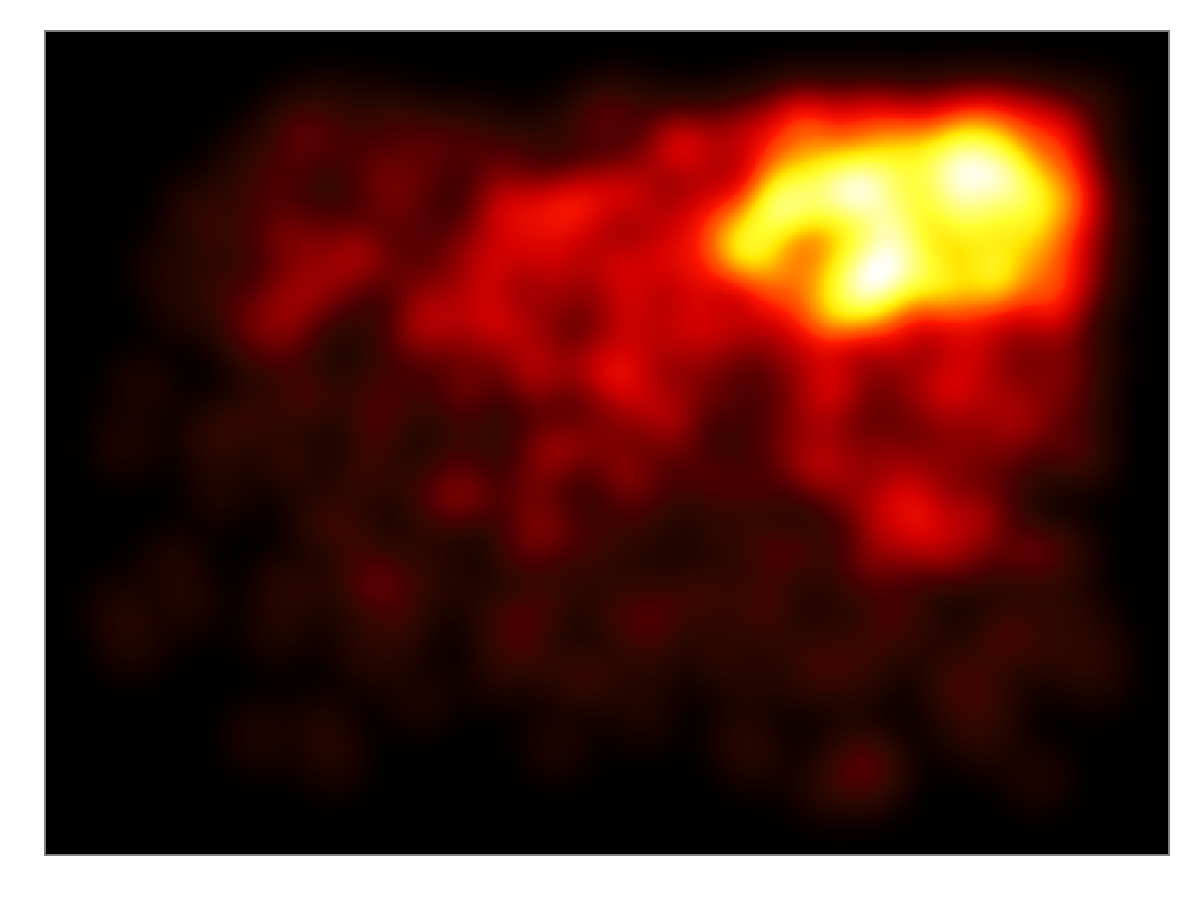
\includegraphics[width=4.2cm]{../scripts/heatmaps/SaccadicFlowMaps/Figures/BBias_13.pdf}}
\subfigure{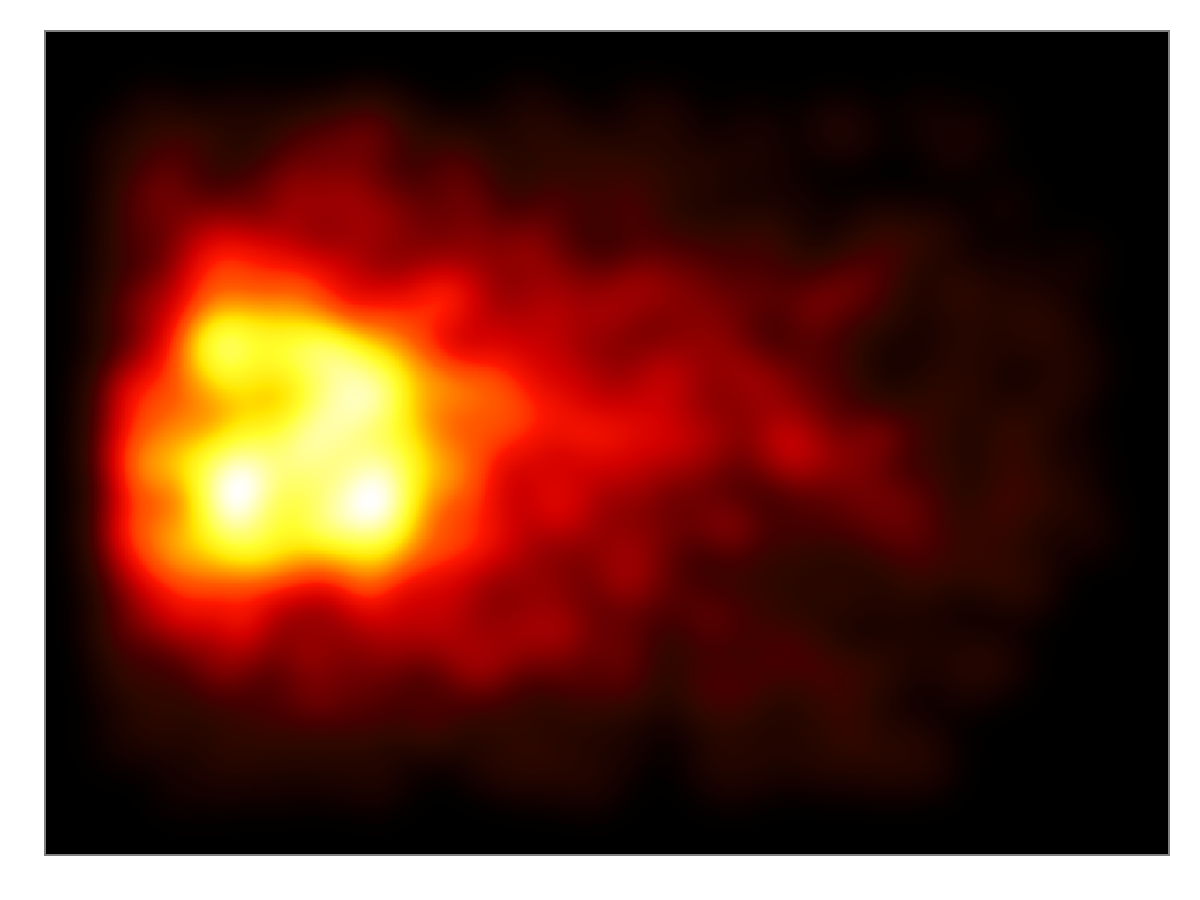
\includegraphics[width=4.2cm]{../scripts/heatmaps/SaccadicFlowMaps/Figures/BBias_21.pdf}}
\subfigure{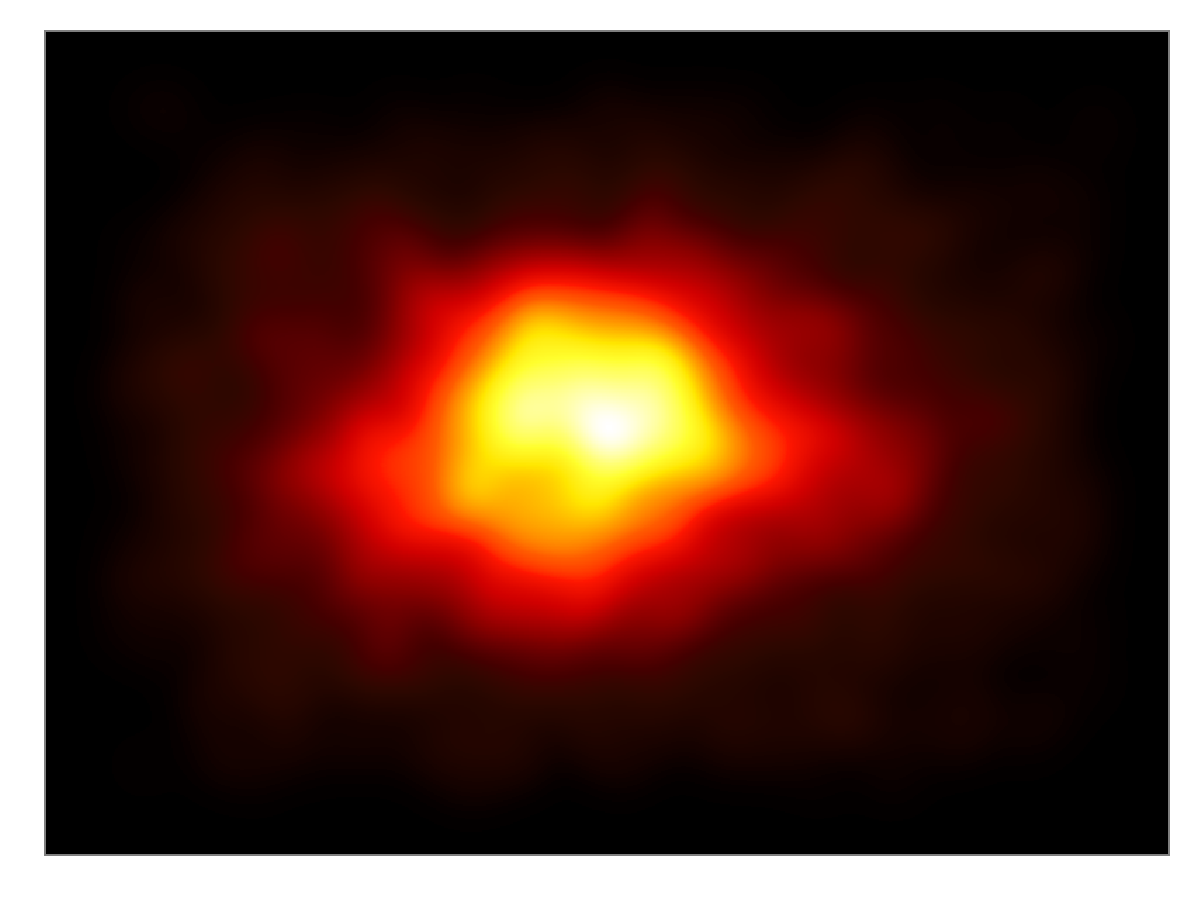
\includegraphics[width=4.2cm]{../scripts/heatmaps/SaccadicFlowMaps/Figures/BBias_22.pdf}}
\subfigure{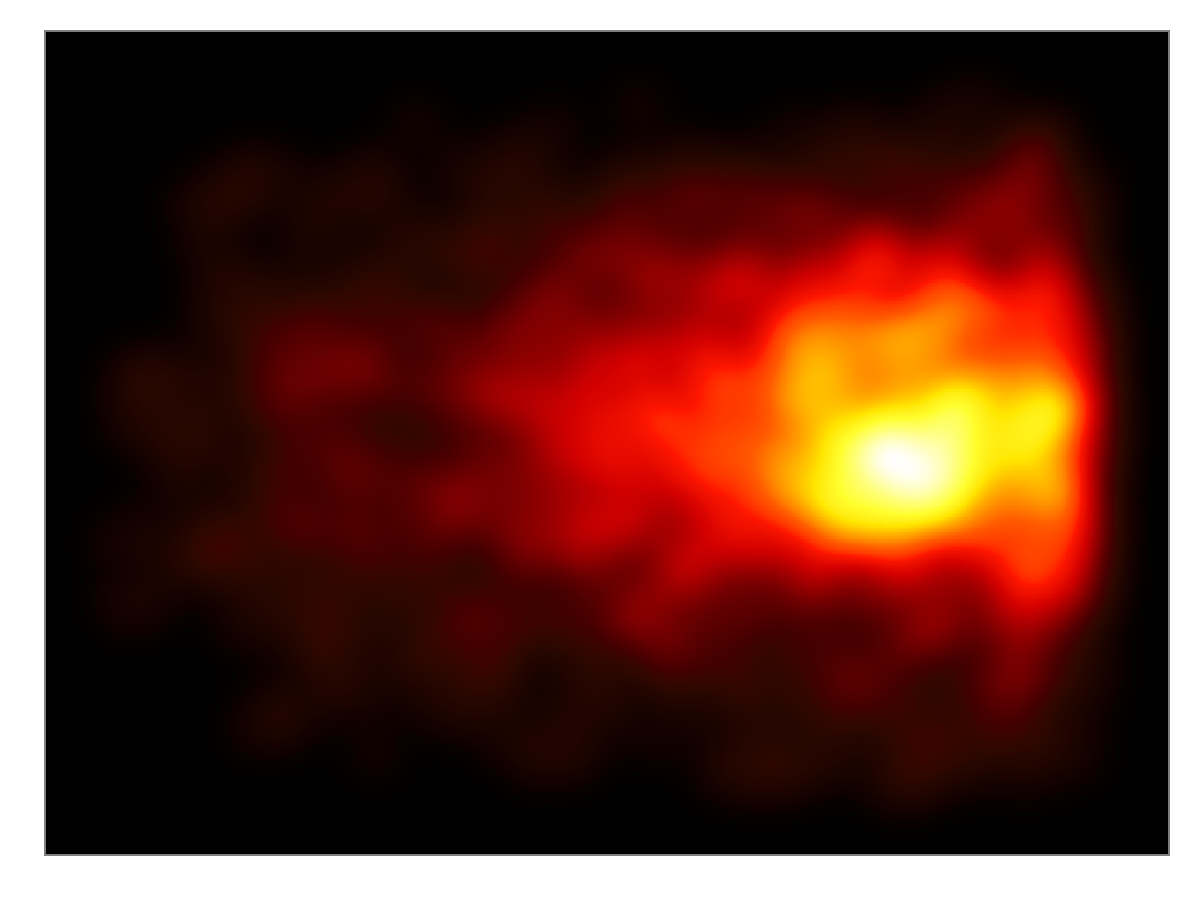
\includegraphics[width=4.2cm]{../scripts/heatmaps/SaccadicFlowMaps/Figures/BBias_23.pdf}}
\subfigure{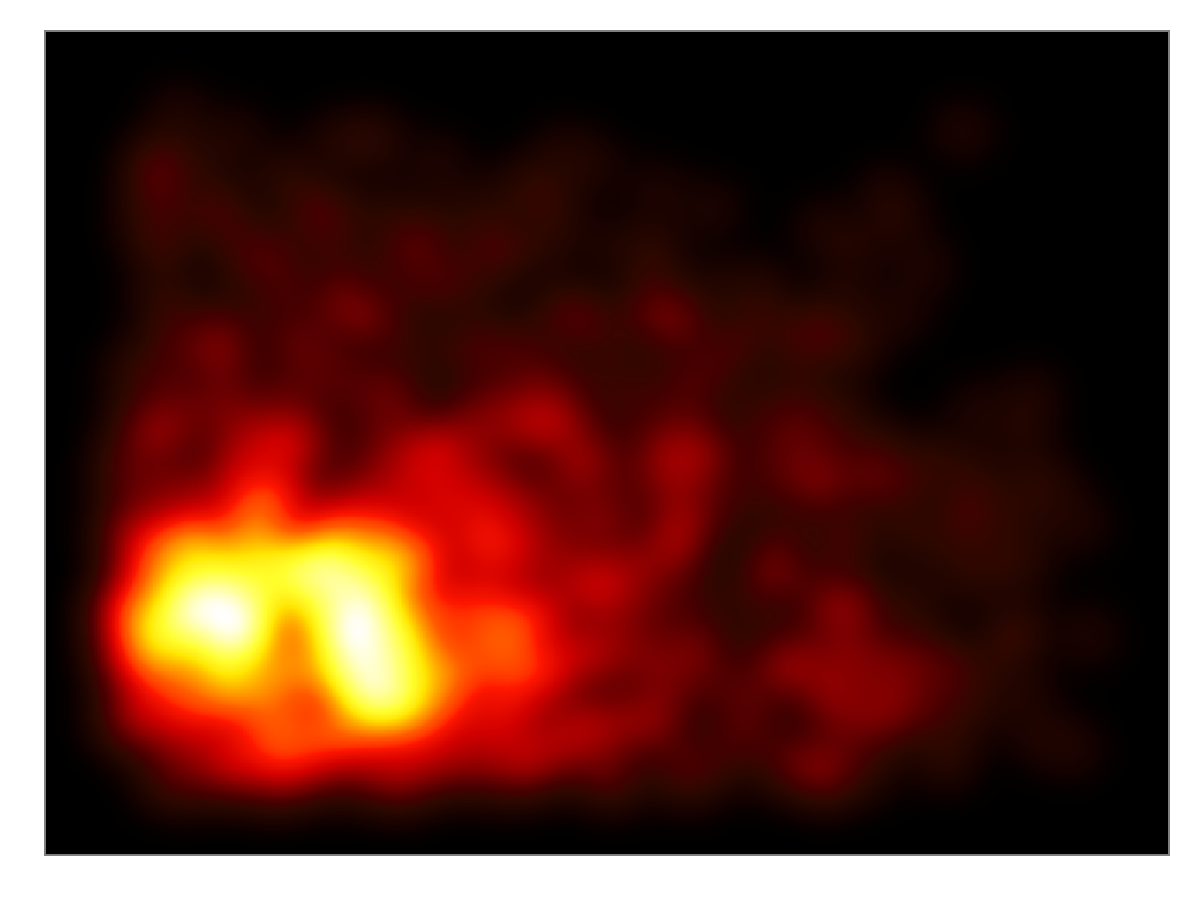
\includegraphics[width=4.2cm]{../scripts/heatmaps/SaccadicFlowMaps/Figures/BBias_31.pdf}}
\subfigure{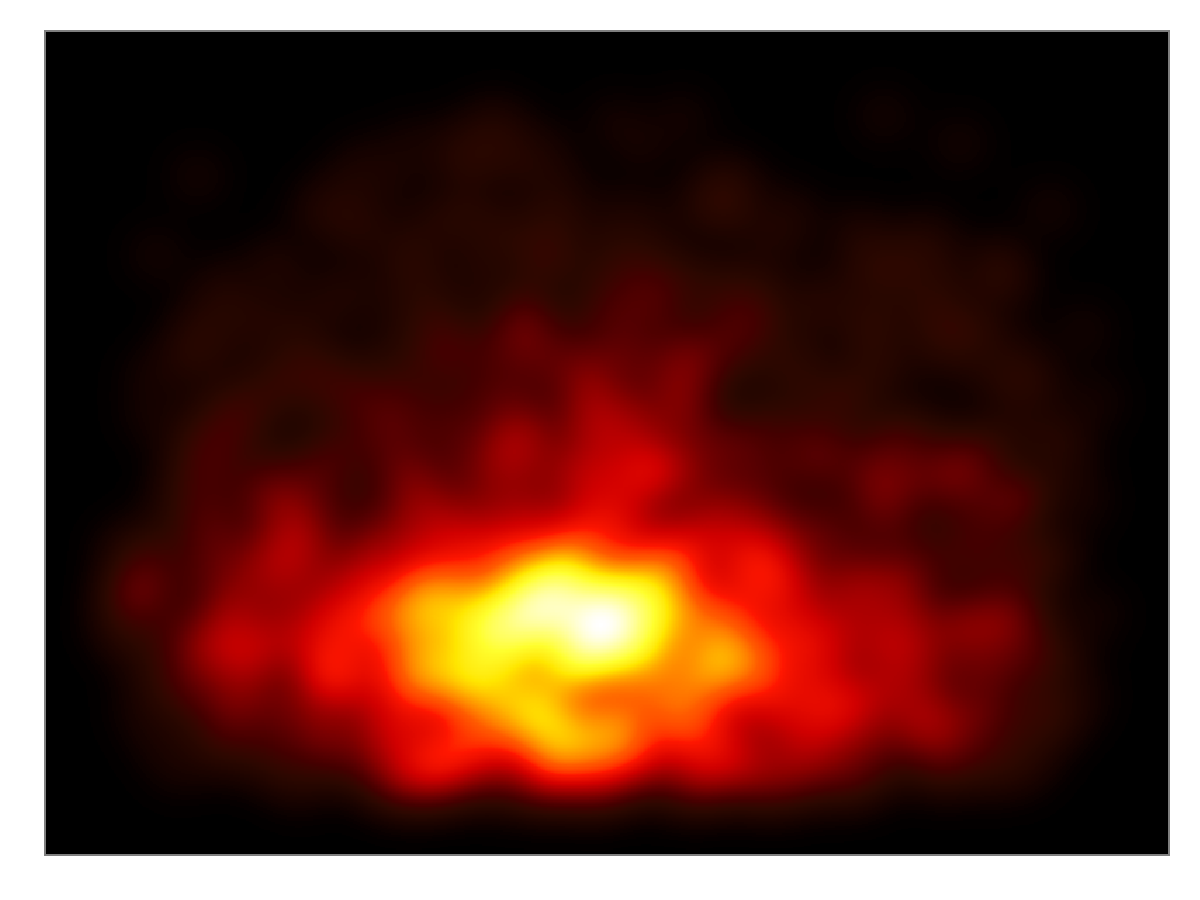
\includegraphics[width=4.2cm]{../scripts/heatmaps/SaccadicFlowMaps/Figures/BBias_32.pdf}}
\subfigure{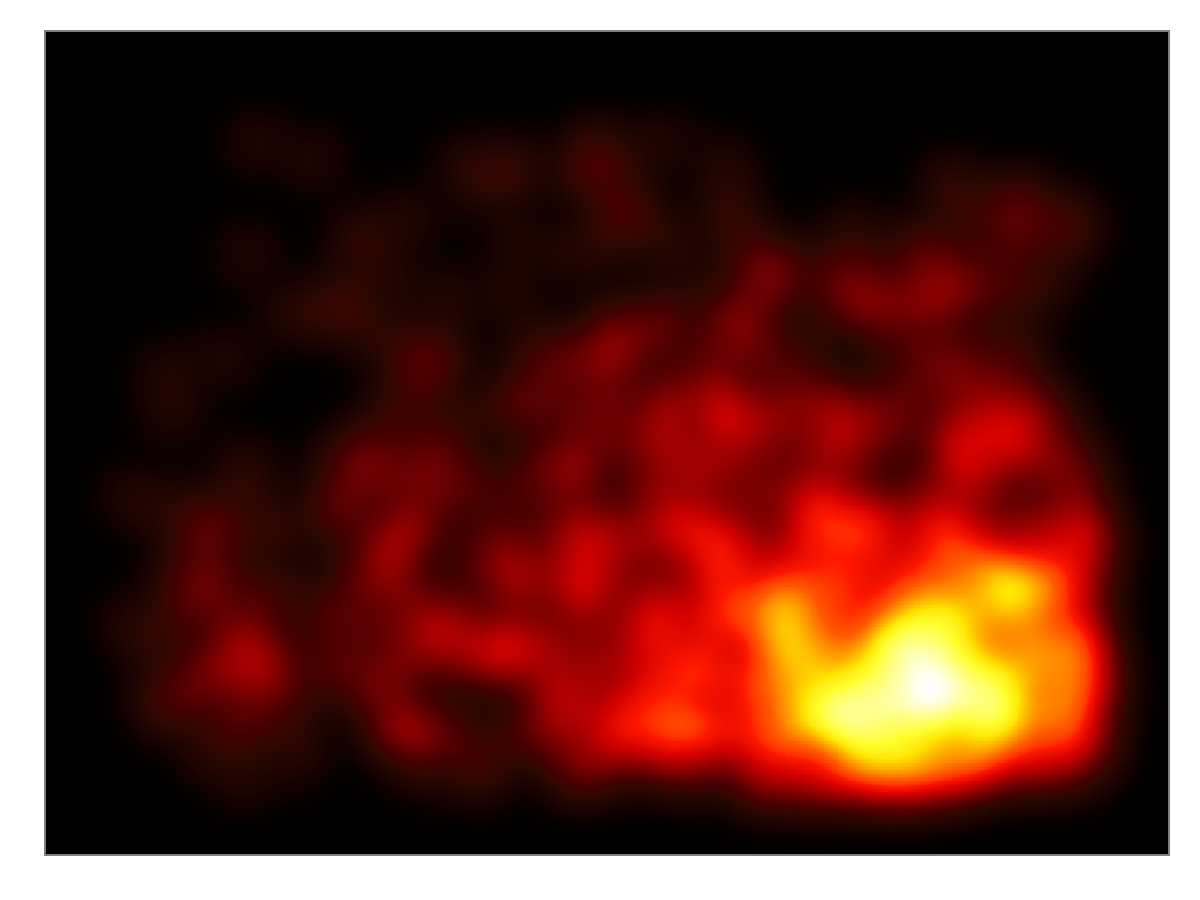
\includegraphics[width=4.2cm]{../scripts/heatmaps/SaccadicFlowMaps/Figures/BBias_33.pdf}}
\caption{Saccade landing positions from fixations that were in different sections of the screen. Data from each plot has been separated into fixations in 9 spatial bins, with the screen being divided into thirds in both horizontal and vertical aspects.}
\label{fig:empiricalSaccadicFlow}
\end{figure*}

%%%%%%%%%%%%%%%%%%%%%%%%%%%%%%%%%%%%%%%%%%%%%%%%%%%%%%%%%%%%%
\subsection{The central bias}
%%%%%%%%%%%%%%%%%%%%%%%%%%%%%%%%%%%%%%%%%%%%%%%%%%%%%%%%%%%%%

There is a strong tendency for people to look close to the centre of pictures \citep{tatler2007,tatler2005, Canosa:2003tu, clarke_tatler2014} and movies \citep{tseng2009} presented on computer screens. There have been a number of suggestions for why this might be. One possibility for this effect is that the muscles of the eye show a preference for the `straight ahead' position, re-centring in the orbit of the eye socket for most comfortable contraction of the ocular muscles (an \emph{orbital reserve} \citep{fuller1996}). As most scene viewing experimental set-ups stabilise the head to increase the accuracy of the eye tracking, and most scenes are presented in the centre of computer displays, such a re-centring mechanism would mean that the centre of images would indeed be preferentially selected. However, when scenes are scrambled into four quadrants, fixations are located near to the centre of each quadrant, rather than the display centre, suggesting that the central tendency is responsive to the viewed content \citep{stainer2013} rather than the frames of the computer monitor.

Another possibility for the central fixation bias is that it represents a \emph{photographer bias} as photographers tend to frame their shots to include the most important content in the centre of the scene. However, when \cite{tatler2007} presented scenes where the image features were biased towards the edge of the scene, the central fixation bias persisted. The final possibility is that as a consequence of repeated exposure to photographer bias, the centre of scenes is simply where people are \emph{trained} to look at images \citep{Parkhurst:2002vo}. Such learning of spatial probabilities of targets can explain why, for example, people tend to look around the horizon when searching for people in natural scenes \citep{birmingham2009, torralba2006, ehinger2009}. Expecting to find interesting content in the centre of scenes might be a consequence of this hypothesis typically being correct. \textbf{The centre is also the best place to look in terms of making best use of parafoveal vision.}

\cite{clarke-tatler2014} revealed that the characteristics of the central bias is remarkably consistent across a series of eye movement databases.... Mention \cite{nuthmann2015} who recently ran this bias on a new dataset and confirmed it accounted for more of the data than an isotropic Gaussian.

\subsection{Other Behavioural biases in saccades}
Further to the observed bias towards the centre of images, it has been revealed that there are underlying biases in the characteristics of eye movement (in terms of the directions and amplitudes of saccades).

\subsubsection{Horizontal Saccades}
It has been noted by several researchers that when viewing scenes, there is a higher proportion of eye movements in horizontal directions than vertical or oblique movements \citep{gilchrist2006,Foulsham2008,tatler-vincent2009, brandt1945, crundeall-underwood1998}. There are a number of possibilities as to why this tendency exists (as discussed in \cite{Foulsham2008}). Firstly, there may be a muscular or neural dominance making oculomotor movements in the horizontal directions more likely. Secondly, the characteristics of photographic images may mean that content tends to be arranged horizontally by the photographer. In such situations, horizontal saccades may be the most efficient way to inspect scenes. Thirdly, using horizontal saccades in scene viewing might be a learned strategy. Observers may learn the natural characteristics of scenes based on previous experience, and therefore demonstrate an increased likelihood of moving in the horizontal direction. A final alternative explanation is that this tendency is a consequence of the aspect ratio of visual displays, which normally allow for larger amplitude saccades in the horizontal than vertical directions \citep{wartburg2007}.

Foulsham and colleagues have presented two interesting exceptions to the horizontal direction bias. \cite{Foulsham2008} found that when the orientation of an image is rotated, the distribution of saccade directions follows the orientation of the scene. A second exception comes from using circular apertures \citep{Foulsham-kingstone2010}. When a scene is presented in a circular aperture, the tendency to make horizontal saccades disappears, being replaced by a tendency to make vertical saccades relative to the image orientation. However, when using fractal images (where images do not have an obvious orientation), observers tend make horizontal saccades, regardless of the angle that the image is presented.

\subsubsection{Coarse-to-fine}

Saccadic amplitudes get shorter and fixation durations get longer over time from scene onset \citep{over2007}. Replicated by \cite{godwin2014} but they offer alternative reasons. And \cite{macinnes2014}
among overs. 


\subsubsection{Leftwards bias}

This falls under the more general spatial attention bias of psuedoneglect \citep{bowers-heilman1980}, which also effects line biesection tasks, etc. \cite{dickinson-intraub2009} found $62\%$ of initial saccades were directed to the left half of the image. Half of the images where mirror reversed to avoid biases in the photographs.

\citep{ossandon2014,nuthmann-matthias2014,learmonth2015,zelinsky1996}. 



\cite{friedrich2014} looked at the effect of native reading direction. 

\subsubsection{Saccadic Momentum and Inhibition of Return}

Several studies have described sequential dependencies during free viewing that bias saccades to repeat the same vector and amplitude (known as saccadic momentum) and to bias saccades away from returning to previously-visited targets (known as inhibition of return). Although both of these phenomena bias fixations away from previously-fixated locations, they differ in that inhibition of return is bound to a location in the search array, i.e. it is coded in object-based or spatiotopic coordinates (e.g. \cite{krueger-hunt2013}), while saccadic momentum has been characterised as a basic tendency to repeat the same motor program \citep{wang2011}. Inhibition of return, unlike saccadic momentum, is task-dependent \citep{dodd2009} and is disrupted by removing the scene or inhibited object  \citep{klein-macinnes1999, takeda-yagi2000}.  \cite{macinnes2014} observed both of these mechanisms operating during free visual search of a complex scene, but presumably only saccadic momentum would be consistently observed for all tasks and images. 

 \cite{macinnes2014, tatler-vincent20xx}

\subsection{Biases and Modelling/Analysis}

These biases, in particular, the central bias, are important to take into account when evaluating the performance of models of fixation location, and investigating relationships between eye movement data and other factors. \textbf{more details and examples}. 

\subsection{The present study}

One of the main contributions of this manuscript is to introduce the \textit{saccadic flow} model. This can be thought of as a generalisation of the central bias: instead of simply characterising the image-independent probability of fixating $(x_i, y_i)$ we model the conditional probabilities $p(x_i,y_i|x_{i-1}, y_{i-1})$. i.e. the probability of making a saccade from to $(x_i,y_i)$ given we are currently fixating $(x_{i-1}, y_{i-1})$.

In Section \ref{sec:usingbiaes} we demonstrate how the central bias and saccadic flow can be used as priors and components of models to improve analysis and visualisation methods. In particular, we will present bias-weighted gaze landscapes, and reanalysis parts of two previously published papers \citep{clarke2013,ehinger2009}. Finally, we will investigate the short-comings of these generative models by comparing synthesised data to human eye movements. 

In Section \ref{sec:biases} we will give full details of the saccadic flow model. Furthermore, we will present an improved central bias distribution and discuss the importance of the left-wards bias (pseudo-neglect).

%%%%%%%%%%%%%%%%%%%%%%%%%%%%%%%%%%%%%%%%%%%%%%%%%%%%%%%%%%
\section{Using Biases}
\label{sec:usingbiaes}
%%%%%%%%%%%%%%%%%%%%%%%%%%%%%%%%%%%%%%%%%%%%%%%%%%%%%%%%%%

This section make use of an improved central bias model (similar to \cite{clarke-tatler2014} except uses a truncated Gaussian distribution to take the image boundaries into account: see Section \ref{sec:truncatedCentral}) and the \textit{saccadic flow} model (described in Section \ref{ModellingFlow}). We present three examples of how these bias models can be used as a prior in order to weight fixations. First of all, we will demonstrate how we can weight fixations in hotspot maps to reduce the noise and give an improved visualisation of the regions of the image that participants looked at more than expect. Secondly, we will re-analyse the effect of attention on object naming from \cite{clarke2013}.  Finally, we will demonstrate how these priors can be used in ROC analysis to improve results. We will re-analyse the effect of the scene context model developed by  \cite{ehinger2009} as an example. 

\subsection{Gaze landscapes}

One technique that is commonly used to visualise the spatial allocation of gaze is to create 'heatmap' plots where colour or luminance are used to indicate the density of fixation on those locations (Figure ~\ref{fig:adjustedHeatmaps}, column 2). Some argue that one problem with visualising data in this way is that they represent all fixations as equal. For example, a fixated location with a fixation of a second would be weighted equally with fixations that lasted half that time. If we want to make an assumption that fixation duration is intimately linked with the importance of that fixation (i.e. we will look longer at more informative information) then we can change our visualisation to weight fixations by their duration (Figure ~\ref{fig:adjustedHeatmaps}, column 3).

One advantage of the \citep{clarke-tatler2014} model, and the saccadic flow model here is that we can represent fixations by the likelihood that they would occur based on the predictions of the models. As there is an image independent tendency to fixate in the centre of the scene (for example), then we might consider that saccades to locations less predicted by these behavioural and oculomotor biases might involve more high-level mechanisms. In Figure ~\ref{fig:adjustedHeatmaps} (column 4 and 5) we present some overlaid heatmap data from the \citep{clarke2013} dataset, where fixations are weighted by the inverse probability of them occurring based on the models of central bias and saccadic flow. These figures reveal that representing data in this manner can allow us to visualise information that was important enough to break the biases of looking at the scene centre, or making saccades in line with our saccadic flow model. We can therefore use this to remove some of the image-independent biases, and reveal the more important image \emph{dependent} information.

\begin{figure*}
\includegraphics[width=\textwidth]{figs/adjustedheatmaps.pdf}
\caption{Traditional 'heat map' plots of fixations normalised by the central bias. This method allows us to characterise fixations that are less accountable for by image-independent central biases.}
\label{fig:adjustedHeatmaps}
\end{figure*}

Or do we call them hotspot maps?

\subsection{Reanalysis of Clarke et al 2013}
\label{sec:reanalysisClarke2013}

In this section we re-analyse the effect of attention on object naming descried in \cite{clarke2013}. In the original study, 24 observers were shown 100 images, with each image displayed for five seconds. After each image had been displayed, observers were asking to name as many objects as they could remember from the scene. The relationship between which objects were named, and where people looked was analysed, along with positional, salience and linguistic features. Several interesting and complex interactions between these different modalities were identified but of particular interest here is the negative interaction between attention and position. This interaction interpreted in terms of the central bias: objects that are central are likely to be looked at more often by default, and hence they will receive a larger attentional scores without actually being more likely to be named.

One of the benefits of using bias functions as priors is that we can re-weight the attentional feature used by \cite{clarke2013} to decorrelate it from object position. By doing so, we can potentially simplify the model and have more intuitive results. 

The attentional feature used by \cite{clarke2013} was based on hotspotmaps, similar to the gaze landscapes presented above. For each object, the attentional score was defined by simply taking the maxima of the pixels in the hotspotmap that fell within the objects boundary. in this reanalysis, we will explore how well attentional features that take the central bias and saccadic flow into account compare to unweighed and fixation duration weighted features. Following the original study, we will repeat our analysis over a range of kernel sizes. 

\subsubsection{Methods}
We will analyse the effect of the different attention features using a glmer.

\subsubsection{Results}

 The results are shown ...

interaction with position

\subsubsection{Discussion}

Discuss and conclude		

\subsection{Reanalysis of Ehinger et al 2009}

We will now explore how our bias distributions can be used to re-analyse the contextual guidance model presented by \cite{ehinger2009}. In their original paper, 14 observers carried out 912 visual searches for a pedestrian in a street scene. These data were used to evaluate computational models of search guidance based on salience, target features and scene context and when combined, these sources of guidance account for $94\%$ of human agreement. The authors also find that scene context offers the most explanatory power. 

In the original analysis, a cross-image control set of fixations was used to account for all the biases within the dataset. While this method is common, there are several issues with it. To start with, we do not know which biases are present in the dataset, and how strong any of them are. The context model developed by \cite{ehinger2009} is based on predicting a horizontal band across the image, which is not all that dissimilar to the central bias disused \cite{clarke-tatler2014}. By taking the central bias into account directly, we can separate out its effects from those of contextual guidance. Finally, the cross-image control method potentially understates the strength of contextual guidance. Visual inspection of the stimuli used in this experiment suggests that most relatively similar to one another (urban street scenes) and one would expect that the context-model should return approximately the same region from one image to the next. If this is a case, this is a data-set wide bias which is of interest to the reader, yet has been removed from the analysis by using a cross-image control set. 

In this section, we will reanalyse the effect of the oracle context maps using ROC curves with three different ways of constructing control points: using a cross-image method, sampling points from the central bias, and sampling points from the saccadic flow model. 

\subsubsection{Methods}

\subsubsection{Results}

\subsubsection{Discussion}


\subsection{Comparison between synthetic and real data}
\label{sec:humanComp}
To what extent does saccadic flow account for coarse-to-fine dynamics? Not that well. Not unexpected.

We can see from Figure \ref{fig:flowHumanComp} that both the central bias and the saccadic flow model do an good job of capturing the distribution of fixation locations in the $x$ and $y$ axes. However, the saccades generated by the flow model tend to be slightly larger than those made by human observers. 

\begin{figure*}[htb]
\centering
\subfigure{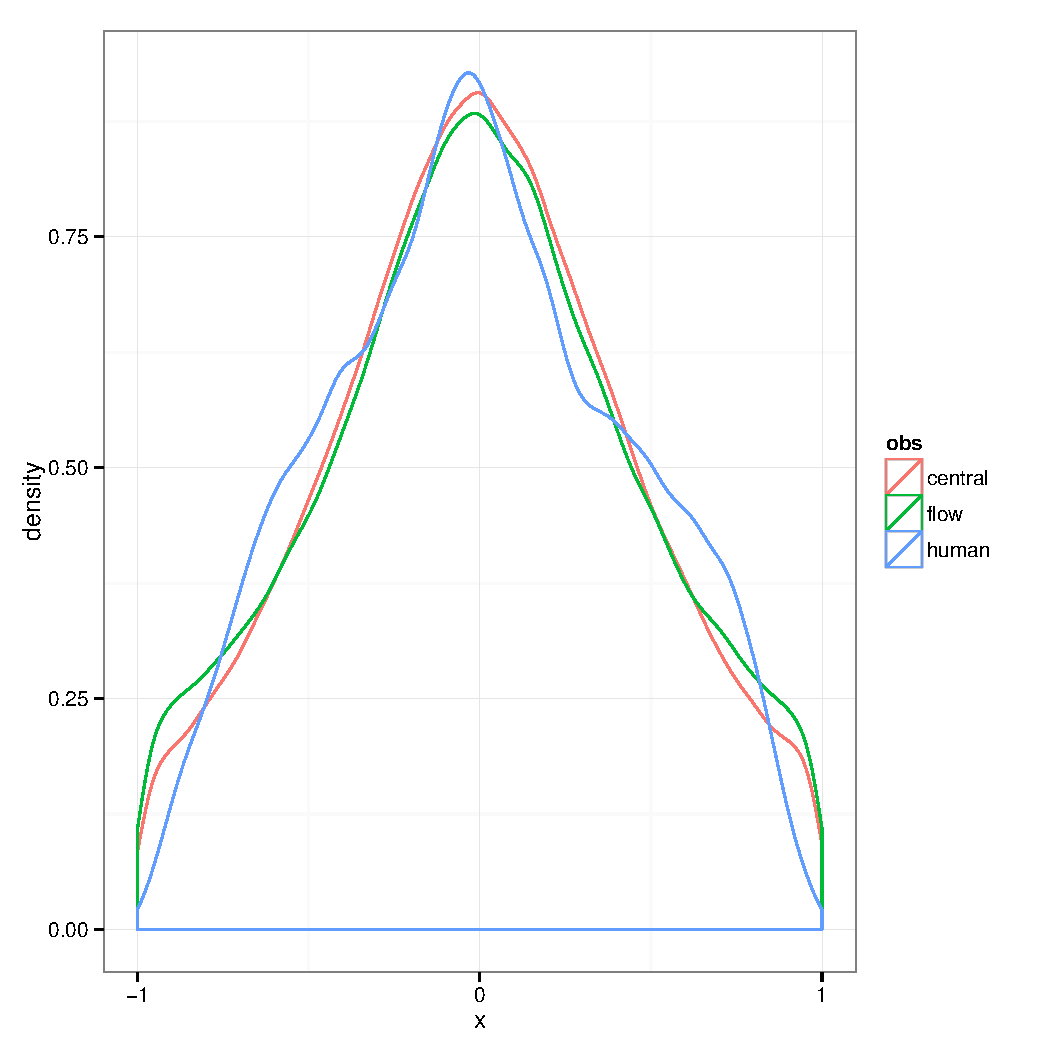
\includegraphics[width=3.8cm]{../scripts/coarse2fine/figs/xFixComparison}}
\subfigure{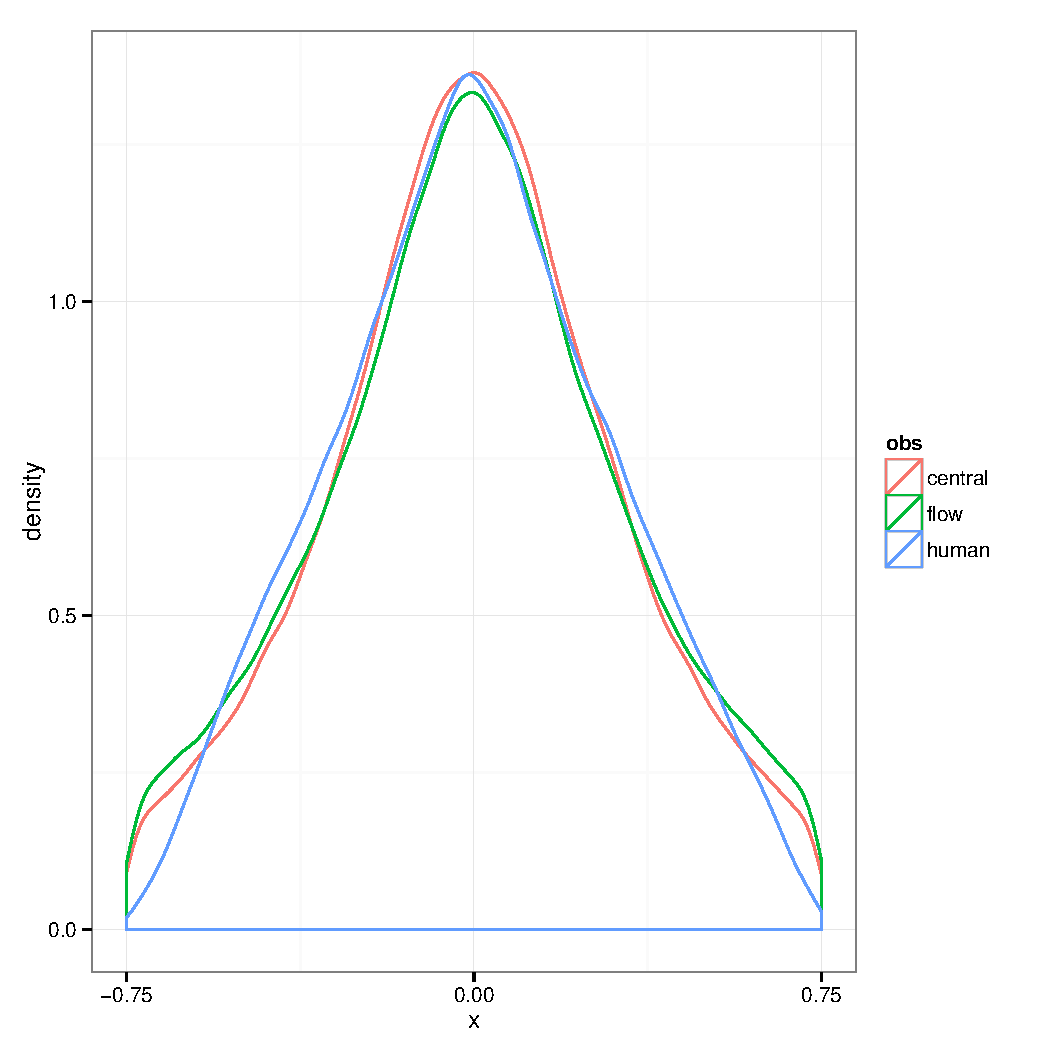
\includegraphics[width=3.8cm]{../scripts/coarse2fine/figs/yFixComparison}}
\subfigure{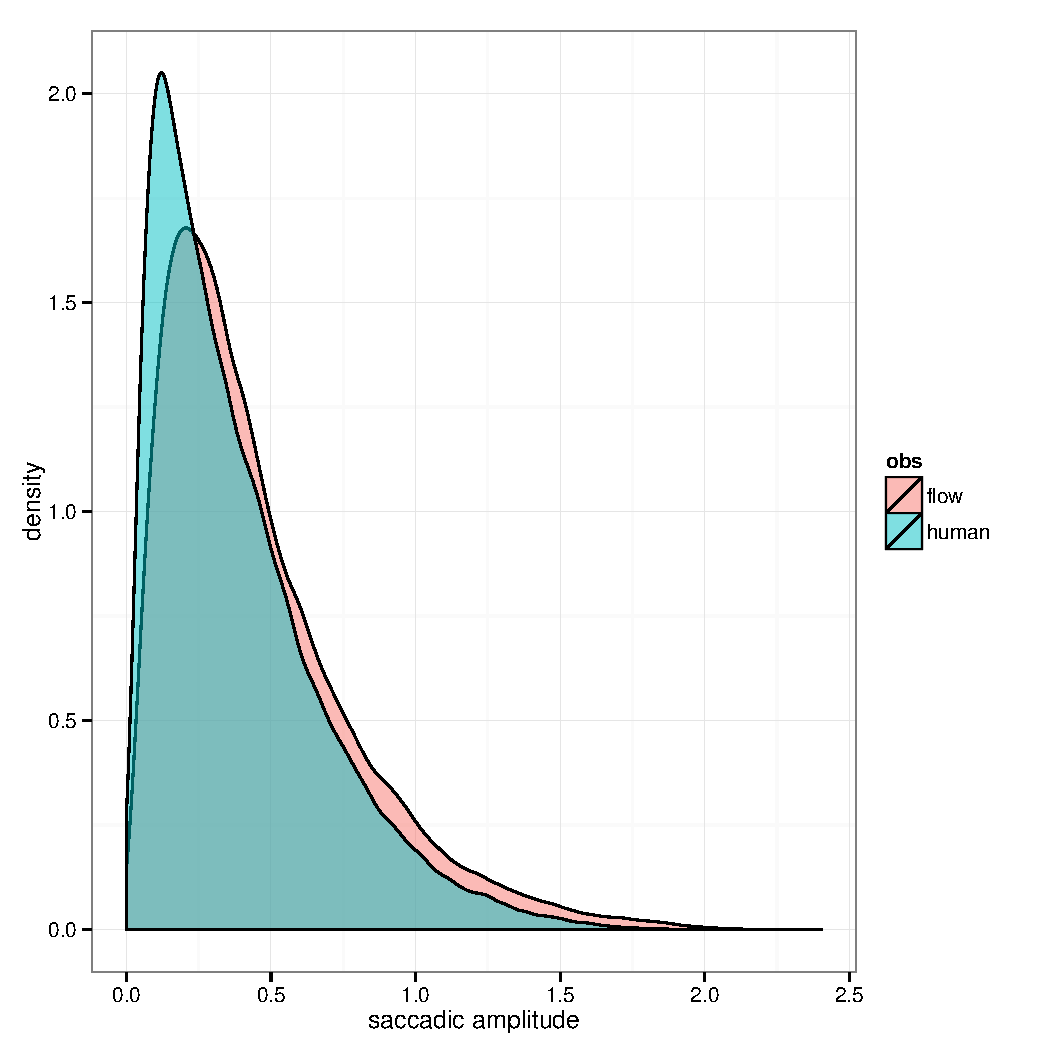
\includegraphics[width=3.8cm]{../scripts/coarse2fine/figs/ampSaccComparison}}
\subfigure{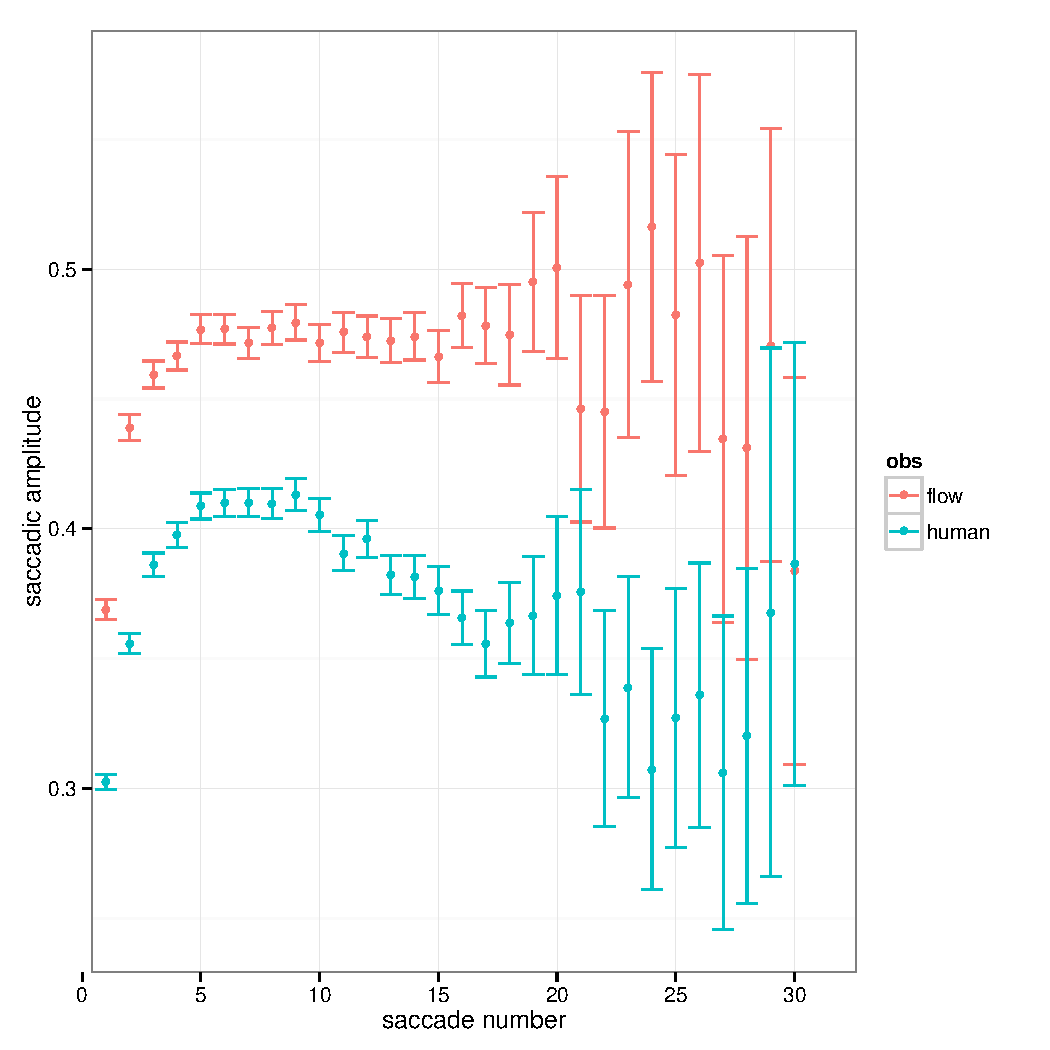
\includegraphics[width=3.8cm]{../scripts/coarse2fine/figs/saccAmpOverTimeFlow}}
\caption{\textit{blue}: human, \textit{red}: central bias, \textit{green}: saccadic flow. \textit{top row}: Comparison of $x$ and $y$ fixation positions between human fixations and synthetic points generated from the central bias and flow model. \textit{bottom row}: We can see that the flow model consistently makes saccades with a slightly larger amplitude than human observers. Distances are expressed relative to the width of the image.}
\label{fig:flowHumanComp}
\end{figure*}

\subsection{Discussion}

We have presented how biases such as saccadic flow and the central bias can be used in different ways. They can be used as a prior on the probability of making saccades to different regions of the image, allowing us to then more clearly visualise the image-dependant behaviour. These bias-weighted gaze landscapes can then be used in analysis as demonstrated in Section \ref{sec:reanalysisClarke2013}.

We can also use the bias distributions to generate data



\section{Modelling Biases}
\label{sec:biases}

In this section, we will present an updated central bias distribution (using a truncated Gaussian); explore the degree of asymmetry in viewing positions, and describe the saccadic flow model. 


%%%%%%%%%%%%%%%%%%%%%%%%%%%%%%%%%%%%%%%%%%%%%%%%%%%%%%%%%%
\subsection{Modelling Methods}
%%%%%%%%%%%%%%%%%%%%%%%%%%%%%%%%%%%%%%%%%%%%%%%%%%%%%%%%%%

In this section, we will give an overview of the methods and data used for the saccadic flow modelling.

\subsubsection{Datasets}

We will uses a number of previously published datasets. The models will be trained on a subset of the 10 datasets used in \cite{clarke-tatler2014}. These data are taken from \cite{clarke2013, tatler2005, tatler2007, yun2013, einhauser2008,judd2009}. The inital saccade after image onset ($9.1\%$ of the data) are excluded, giving us a total of 159,226 saccades. We chose to remove the data from \cite{asher2013} from our training set as the images have an aspect ratio of 5:4, whereas the rest of the data in our training set has an aspect ratio of 4:3. The pedestrian search dataset \citep{ehinger2009} was removed from the training set as previous analysis \citep{clarke-tatler2014} shows that it appears to be biased compared to the other datasets. Both these datasets are now used as test sets to evaluate how well our models generalise. 

We also add a number of other datasets to our test suite collection. 
\begin{itemize}

\item \cite{jiang2014} collected data from 16 observers viewing 500 natural scenes containing crowds of people (aspect ratio 4:3).

\item \cite{clarke2009} has a dataset of fixations made during a visual search for a target on a homogeneous textured background (i.e. target in noise). This dataset differs from the previous in that there is no semantic image content in the scene, and the stimuli had a 1:1 aspect ratio.

\item \cite{greene-wolfe2012} released a dataset of observers viewing square greyscale photographs.

\item \cite{borji2015} recently released a very large ($\approx 0.625$million fixations, 2000 images) dataset collected over twenty different stimuli types. Given the size of this dataset, and the widescreen 16:9 aspect ratio, the evaluations on this dataset are presented seperately, and split by stimuli class.

\end{itemize}

An overview of the datasets used is given in Appendix Tables \ref{tab:datasets} and \ref{tab:setuptable}.

\subsubsection{Pre-processing}

As with \cite{clarke-tatler2014} we have normalised all fixations to the image frame, keeping the aspect ratio constant. ie, $(x,y)\in (-1.-1)\times(-a,a)$ with typically $a=0.75$. The initial fixations and saccades were not included in the analysis. Saccades with a start or end point falling outside of the image frame were also removed. 

When fitting saccadic flow models,  we \textit{mirrored} the set of fixations, but adding in reflected copies of the data (reflected in the horizontal, vertical and both midlines). This has two advantages. (i) It is an easy way to make saccadic flow biases in the horizontal or vertical directions. This is similar to how the central bias was defined \cite{clarke-tatler2014}, but by a different mechanism (with the central bias, the model fitting procedure is much simpler and so we just enforced zero mean and 0s in the covariance matrix). (ii) It increases the amount of data available for fitting by a factor of four. This is important as (due to the central bias) there are relatively few saccades that originate from the corners of the images. By equating all corners, we can pool the data and obtain more stable estimates for the underlying distribution. 


The downside of mirroring saccades in this manner is that our model of saccadic flow will be insensitive to the \textit{leftwards} bias in natural scene viewing \citep{nuthmann-matthias2014}. This will be discussed in Section \ref{sec:LeftRight}. Similary, as ignore the timecourse of saccades we will not capture \textit{corase-to-fine} dynamics (discussed previous in Section \ref{sec:humanComp}).

We will model and discuss saccadic flow, coarse-to-fine, and left v right. 

\subsection{Truncated Central Bias}
\label{sec:truncatedCentral}
First, we will update the central bias from \cite{clarke-tatler2014} and use a truncated normal distribution. This is very straight forward. Re-fitting a multivariante gaussian to the data reduces the deviance in the central bias model by $4.4\%$. Usng a truncated Gaussian gives us an improvement of $12\%$. We can round the truncated Gaussian model to $\mu = (0,0)$, with a covariance matrix of $(0.32, 0; 0, 0.144)$ with no loss of precision. i.e. this is identical to \cite{clarke-tatler2014} except with $\sigma=0.32$ rather than $0.22$

\subsection{Left v Right}
\label{sec:LeftRight}

Initially more fixations to the left half of the image \citep{nuthmann-matthias2014}. We replicate this here (Figure \ref{fig:leftrightDist}).

\begin{figure}
\centering
\subfigure{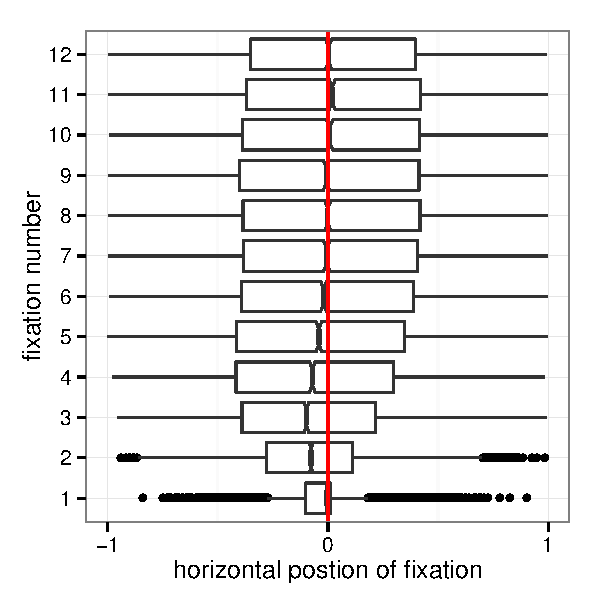
\includegraphics[width=3.8cm]{../scripts/leftVright/graphs/leftrightbias.pdf}}
\subfigure{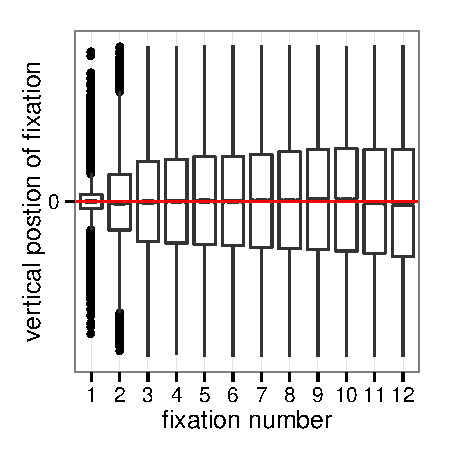
\includegraphics[width=3.8cm]{../scripts/leftVright/graphs/updownbias.pdf}}
\caption{Distribution of horizontal and vertical fixations by fixation number.}
\label{fig:leftrightDist}
\end{figure}

However, it has only a very small effect on explaining the varition over whole datasets: fitting an ANOVA to predict the $x$ coordinates of the fixations given the fixaiton number gives adjusted $R^2=0.004$. If we limit our analysis to the first 5 fixations in each scanpath, this only increases to adjusted $R^2=0.01$. 

Hence we will ignore this effect from now on. By treating everything as symmetrical, we lose very little explanitory power, while restricitng the number of parameters, or increasing the amount of data available (by mirroring fixations). 

\subsection{Saccadic Flow}
\label{ModellingFlow}

Saccadic flow can be thought of as a generalisation of the central bias. Instead of computing the distribution of all saccadic endpoints in a dataset, we look at the distribution of saccade endpoints given the start points. So for a saccade from $(x_0, y_0)$ to $(x_1, y_1)$ we want to model $p(x_1,y_1|x_0, y_0)$ This is illustrated in Figure \ref{fig:empiricalSaccadicFlow}.

\subsubsection{Modelling}


To characterise how the distribution of saccadic endpoints varies with the start point, we used a sliding window approach. All saccades that originated in a $n\times n$ window were taken and used to fit a multivariate Gaussian distribution. This window was then moved over the stimuli in steps of $s=0.01$. Parameter sets estimated from windows containing less than 250 datapoints were removed. Multivariate polynomial regression was then used to fit 4-th order polynomials to each of the parameters. Robust estimation was used (\texttt{rlm} from the texttt{MASS} library) to stop the model fits being overly infleunced by outlier points from the image boundary. We experimented with varying the window size ($n\in\{0.05,0.1, 0.2\}$). However, as this parameter was found to have a negligible result, we only report the results for $n=0.05$.

\subsubsection{Results}

Figure \ref{fig:nParamsOverSpace} shows how the parameters for the multivariate Gaussian distribution vary over horizontal position for a selection of vertical positions. The regression coefficients (given in supplementary materials) allow us to estimate the conditional probability of a saccade to $(x_1, y1)$ given the starting fixation $(x_0, y_0)$.

\begin{figure*}
\centering
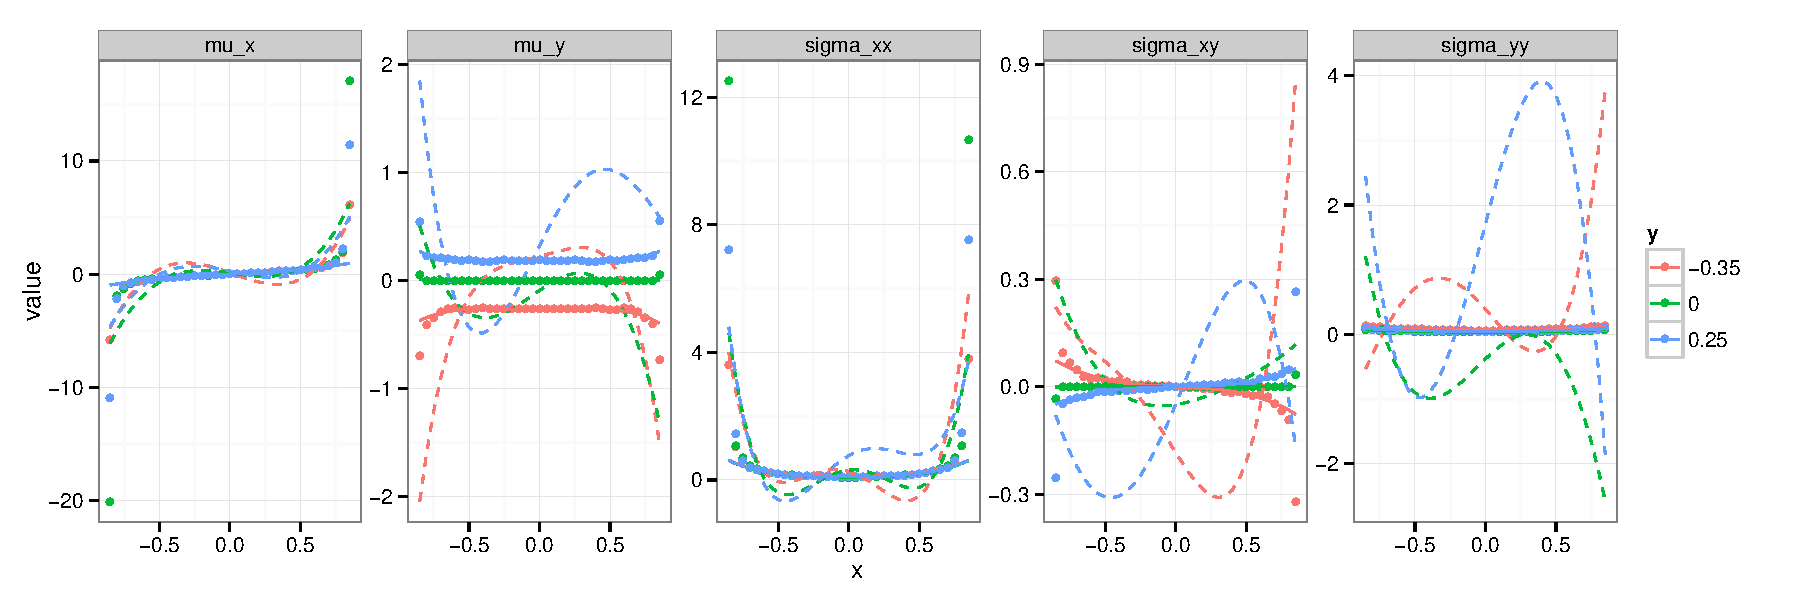
\includegraphics[width=16cm]{../scripts/flow/figs/NparamsChagingOverSpace_ALL_tN}
\caption{How the truncated Gaussian parameters vary with saccadic starting location. Dotted line show polynomial regression fits, solid line shows robust polynomial regression.}
\label{fig:nParamsOverSpace}
\end{figure*}


How well does this model account for the fixations in our datasets? Figure \ref{fig:nFlowDevAll} shows the deviance of the flow model expressed as a proportion of the deviance of the Clarke-Tatler central bias. For reference, we also show the results for re-fitting the central bias to each dataset. From this figure, we can see that the flow-normal model approximately halves the deviance. 

\begin{figure*}
\centering
 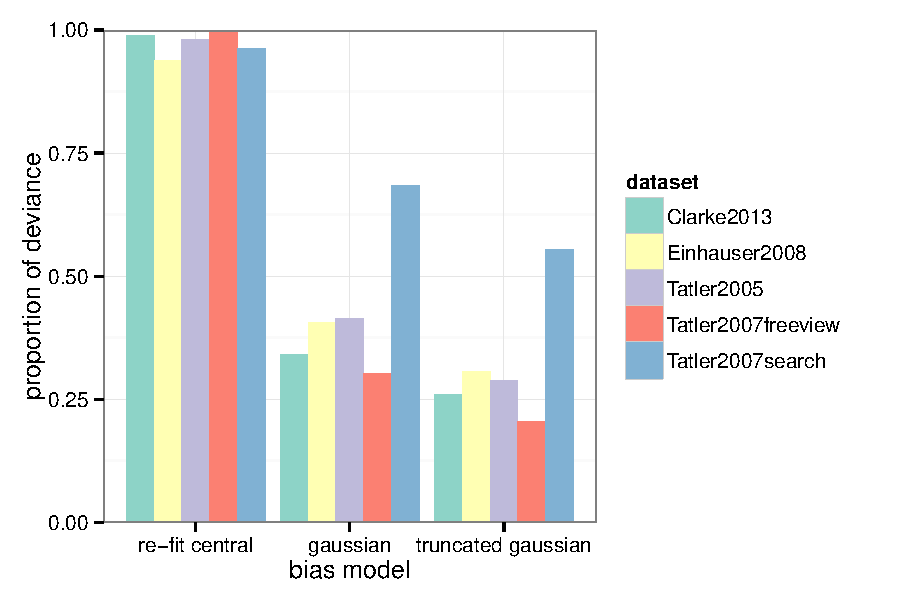
\includegraphics[width=12cm]{../scripts/flow/figs/llh_ALL.pdf}
\caption{Flow:normal log likelihood results. We can see that re-fitting the central-bias to each specific dataset offers little improvement over using the Clarke-Tatler model, while the flow model offers a substantial improvement.}
\label{fig:nFlowDevAll}
\end{figure*}

As the flow:normal model is significantly more complex, requiring nine times as many parameters, it is important to test for robustness. We can test how well our model generalises on testing it on other datasets, for example, \cite{borji2015}. 


\begin{figure*}
\centering
 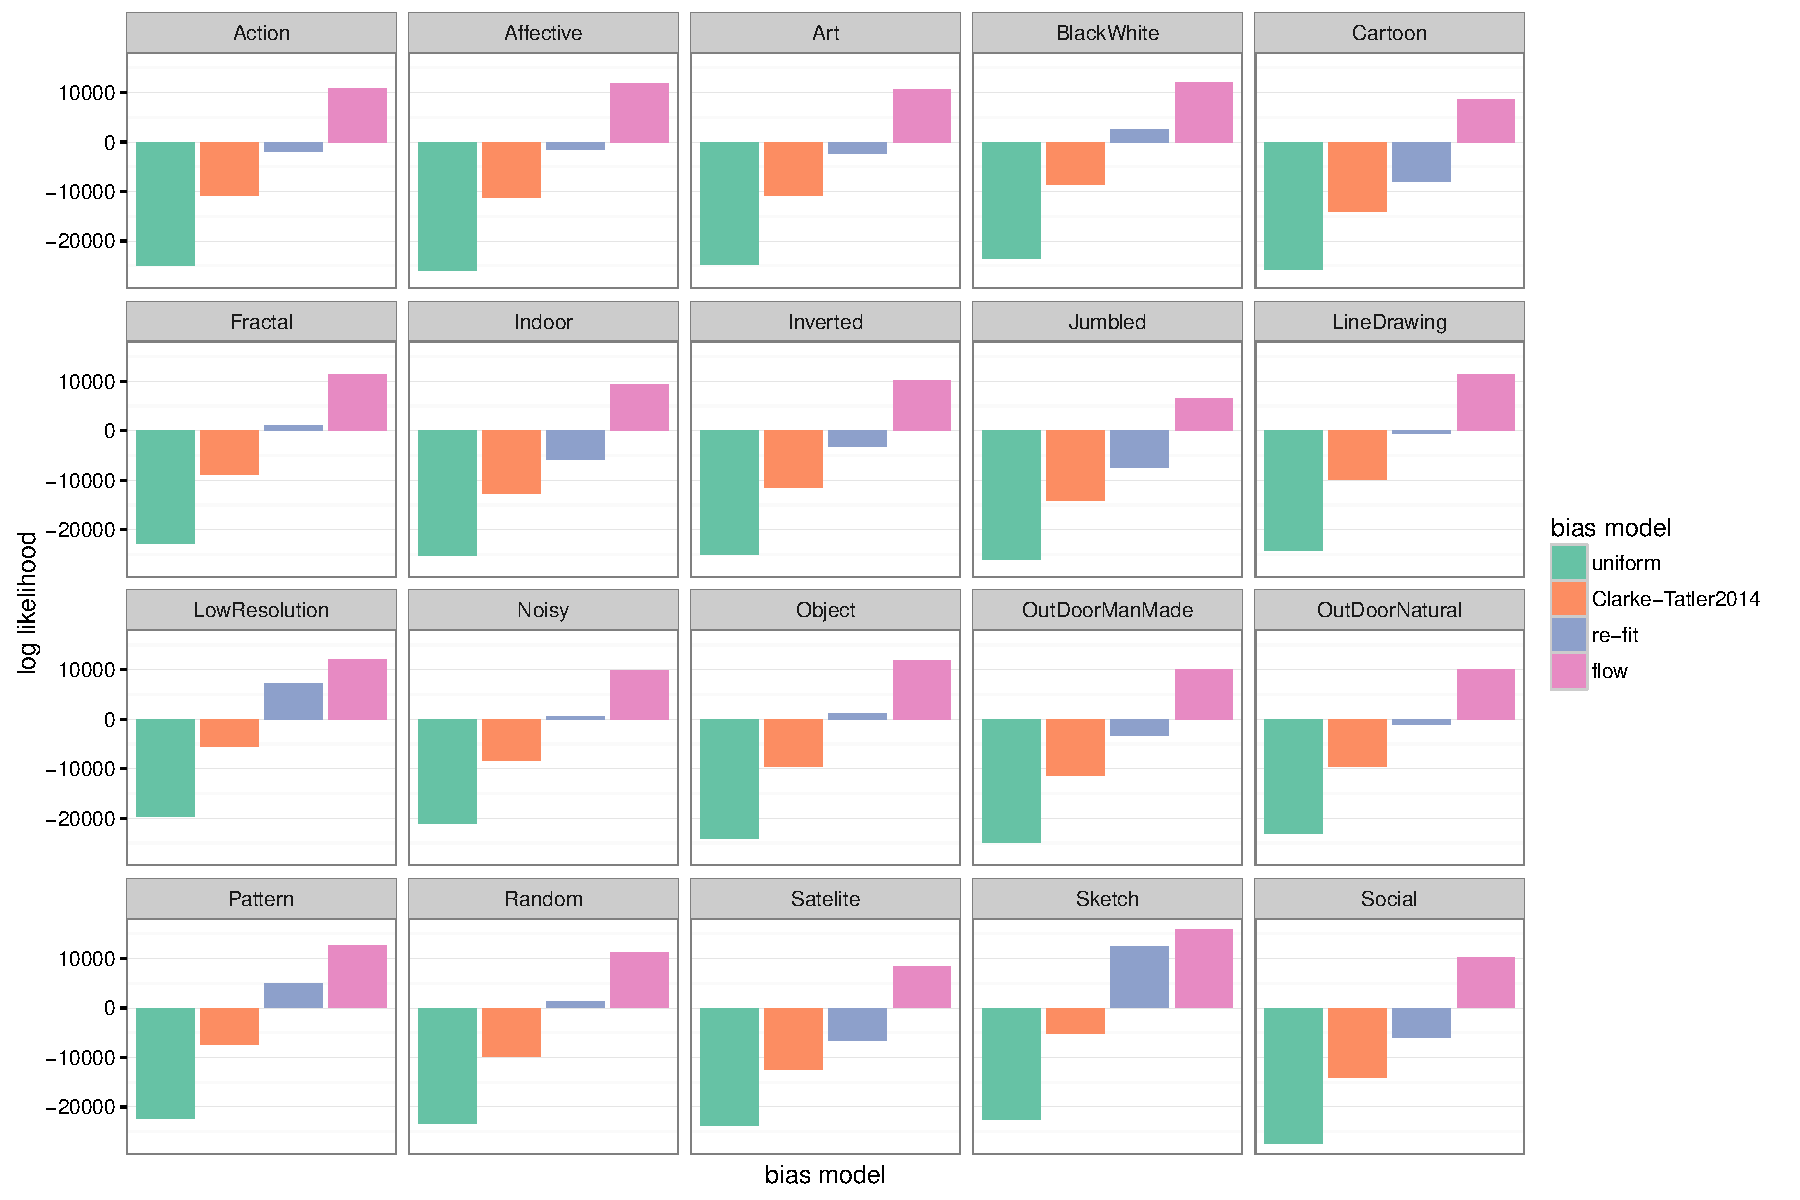
\includegraphics[width=12cm]{../scripts/flow/figs/llh_Borji.pdf}
\caption{Flow:normal deviance results. We can see that re-fitting the central-bias to each specific dataset offers little improvement over using the Clarke-Tatler model, while the flow:normal model decreases the deviance by half.}
\label{fig:nFlowDevBorji}
\end{figure*}

% \begin{figure}
% \centering
%  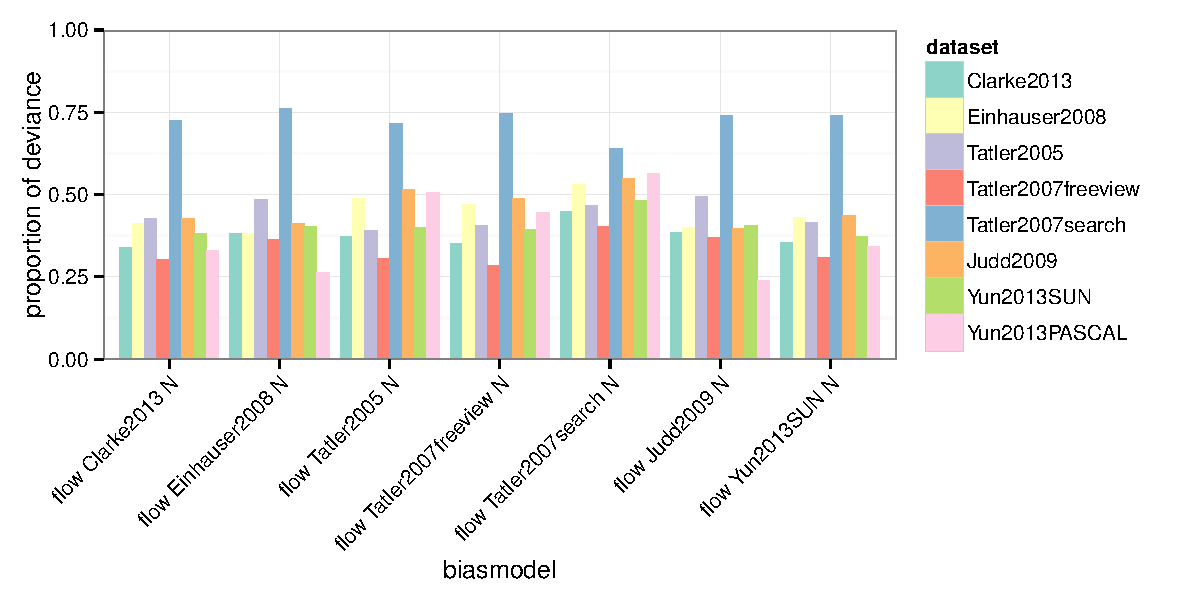
\includegraphics[width=12cm]{../scripts/flow/figs/llh_crossDataset.pdf}
% \caption{Flow:normal deviance results over datasets. In general, we can see that bias models trained on different datasets all explain around the same amount of variance in the datasets.}
% \label{fig:nFlowDevCross}
% \end{figure}

\subsubsection{Discussion}

We put the Flow:normal model forward as a robust prior for image-content independent saccadic behaviour. This model can be thought of as as partner of the Clarke-Tater central bias, and we expect that in some cases, the simpler central bias will be more appropriate, while in others, the more complex flow model is a better choice. We have demonstrated that although this model requires more parameters, it generalises well from one dataset to another and is a far better baseline for modelling a scan-path than the central bias.

There are two main simplifications to our modelling work. First of all, we are using an unbounded distribution (ie, $(x,y)\in \mathbb{R}^2$) to model bounded data. While it is possible to deal with this issue, by either applying a transform $(-1,1)\rightarrow \mathbb{R}$ (such as $z=log(\frac{x'}{1-x'})$, where $x'=\frac{x+1}{2}$), or fitting a truncated multivariate Gaussian, we decided that given the good performance of the model as is, it was not worth adding the additional complexities to our model at this time. 

The second simplification is that we are treating the data as normal. From Figure \ref{fig:empiricalSaccadicFlow} we can see that the data is clearly skewed, particularly in the corners. We will attempt to address these issues in the following section.

\section{Discussion}


What isn't captured by our flow model? There will be some stuff in \cite{macinnes2014}

\subsection{Scenes and natural viewing behaviour}
That observers organise their viewing behaviour on computer screens around the reference frames provided by the bounds of scenes (see also \cite{Stainer:2013ce}) causes problems for relating findings of eye guidance in scenes to eye guidance in natural behaviour, as the bounds of such reference frames are unclear in the real world. While it has been suggested that we tend to fixate near to the centre of our `straight ahead' head position [FOULSHAM WALKING, CRISTINO AND BADDELEY?], there are no discrete edges as are typical in computer based scene viewing paradigms. If fixation locations are constrained by the bounds of the scene, this highlights the care we must take about the generalisations we make from findings in the lab to the real world (see [kingstonepaper 2010]). 


\section*{Acknowledgements}

%Thanks to Adelchi Azzalini for advice on using the \texttt{sn} package for \texttt{R}. And mention grants. 

\appendix
\section{Dataset Details}

Here are all the details on the datasets used in this paper. (Table \ref{tab:datasets} and \ref{tab:setuptable}).


\begin{table*}
\centering
\small
\begin{tabular}{l|llll}
 						& Observers & Images &  Task & Display duration\\
\hline
\cite{clarke2013}     	& 24   	& 100   & object naming & 5000 ms\\
\cite{yun2013} - SUN    & 8     & 104   & image description & 5000 ms\\
\cite{tatler2005}     	& 14    & 48    & memory 			& variable\\
\cite{einhauser2008} 	& 8		& 93    & object naming 	& 3000 ms \\
\cite{tatler2007} - free & 22   & 120   & free viewing      & 5000 ms\\
\cite{judd2009}         & 15 	& 1003  & free viewing 		& 3000 ms\\
\cite{yun2013} - PASCAL & 3 	& 1000  & free viewing 		& 3000 ms\\
\cite{tatler2007} - search & 30 & 120	& visual search 	& 5000 ms\\
\hline
\cite{clarke2009} 		& 7		& 360	& visual search 	& variable\\
\cite{ehinger2009}     	& 14 	& 912 	& visual search 	& variable\\
\cite{asher2013}    	& 25    & 120   & visual search		& variable\\
\cite{jiang2014}  		& 16 	& 500 	& free viewing  	& 5000 ms \\
\cite{borji2015}  		& 120	& 4000  & free viewing		& 5000 ms\\
\end{tabular}

\caption{Summary of the 13 datasets used throughout this study. The top eight datasets were used to train the model, while the bottom five were only used for evaluation.}
\label{tab:datasets}
\end{table*}

\begin{table*}
\begin{center}
\small
\begin{tabular}{l|llllll}
 & Eye tracker & \vtop{\hbox{\strut Viewing}\hbox{\strut distance}}
 & \vtop{\hbox{\strut Screen}\hbox{\strut size}}
 & \vtop{\hbox{\strut Image}\hbox{\strut size}}
 & \vtop{\hbox{\strut Viewing}\hbox{\strut angle}}
 & \vtop{\hbox{\strut Chin /}\hbox{\strut head rest}}\\
\hline
\cite{tatler2005} 			& EyeLink I 	& 60 cm 	& 17" 	& $800 \times 600$ 	& $30 \times 22^{\circ}$ 	& no\\
\cite{tatler2007} - free 	& EyeLink II 	& 60 cm 	& 21" 	& $1600 \times 1200 $	& $40 \times 30^{\circ}$ 	& no \\
\cite{tatler2007} - search 	& EyeLink II 	& 60 cm 	& 21" 	& $1600 \times 1200$ 	& $40 \times 30^{\circ}$ 	& no\\
\cite{einhauser2008} 		& EyeLink 1000 	& 80 cm 	& 20" 	& $1024 \times 768$ 	& $29 \times 22^{\circ}$ 	& yes\\
\cite{judd2009} 			& ? 			& 2 feet 	& 19" 	& $1024 \times 768*$ 	& ? 				& yes\\
\cite{clarke2013} 			& EyeLink II 	& 50 cm 	& 21" 	& $800 \times 600$ 	& $31 \times 25^{\circ}$ 	& no\\
\cite{yun2013} - PASCAL 	& EyeLink 1000	& ? 		& ? 	& ? 			& ? 				& ?\\
\cite{yun2013} - SUN 		& EyeLink 1000 	& ? 		& ? 	& ? 			& ? 				& ?\\
\hline
\cite{clarke2009} 			& Tobii x50 	&87 cm			& 20"		& $1024\times 1024$	&	$16.7\times16.7^{\circ}$ & yes \\
\cite{ehinger2009} 			& ISCAN RK-464 	& 75 cm 	& 21" 	& $800 \times 600$ 	& $23.5 \times 17.7^{\circ}$& yes\\
\cite{asher2013} 			& EyeLink 1000 	& 55 cm 	& ? 	& $1024 \times 1280$& $37.6 \times 30.5^{\circ}$& yes\\
\cite{jiang2014}  			& Eyelink 1000 	& 57 cm		& 22"	& $1024 \times 768$ & $38.8 \times 29.1^{\circ}$& ?\\
\cite{borji2015} 			& Eyelink 1000	& 106 cm	& 42" 	& $1920\times1080 $	&$45.5\times31^{\circ}$& yes \\
\end{tabular}
\end{center}

\caption{Details of the experimental setups in each of the 10 datasets analysed in the present study. We provide only information reported in the original articles. Question marks indicate information not reported in the original article. *For the Judd et al dataset images varied in pixel dimensions but the majority were at 1024 x 768.}
\label{tab:setuptable}
\end{table*}

\bibliographystyle{plainnat}
\small
\bibliography{literature}
\end{document}